\begin{figure*}[ht]
  \centering
  \subfloat[][Average Scores w/ StDev Error Bars]{
    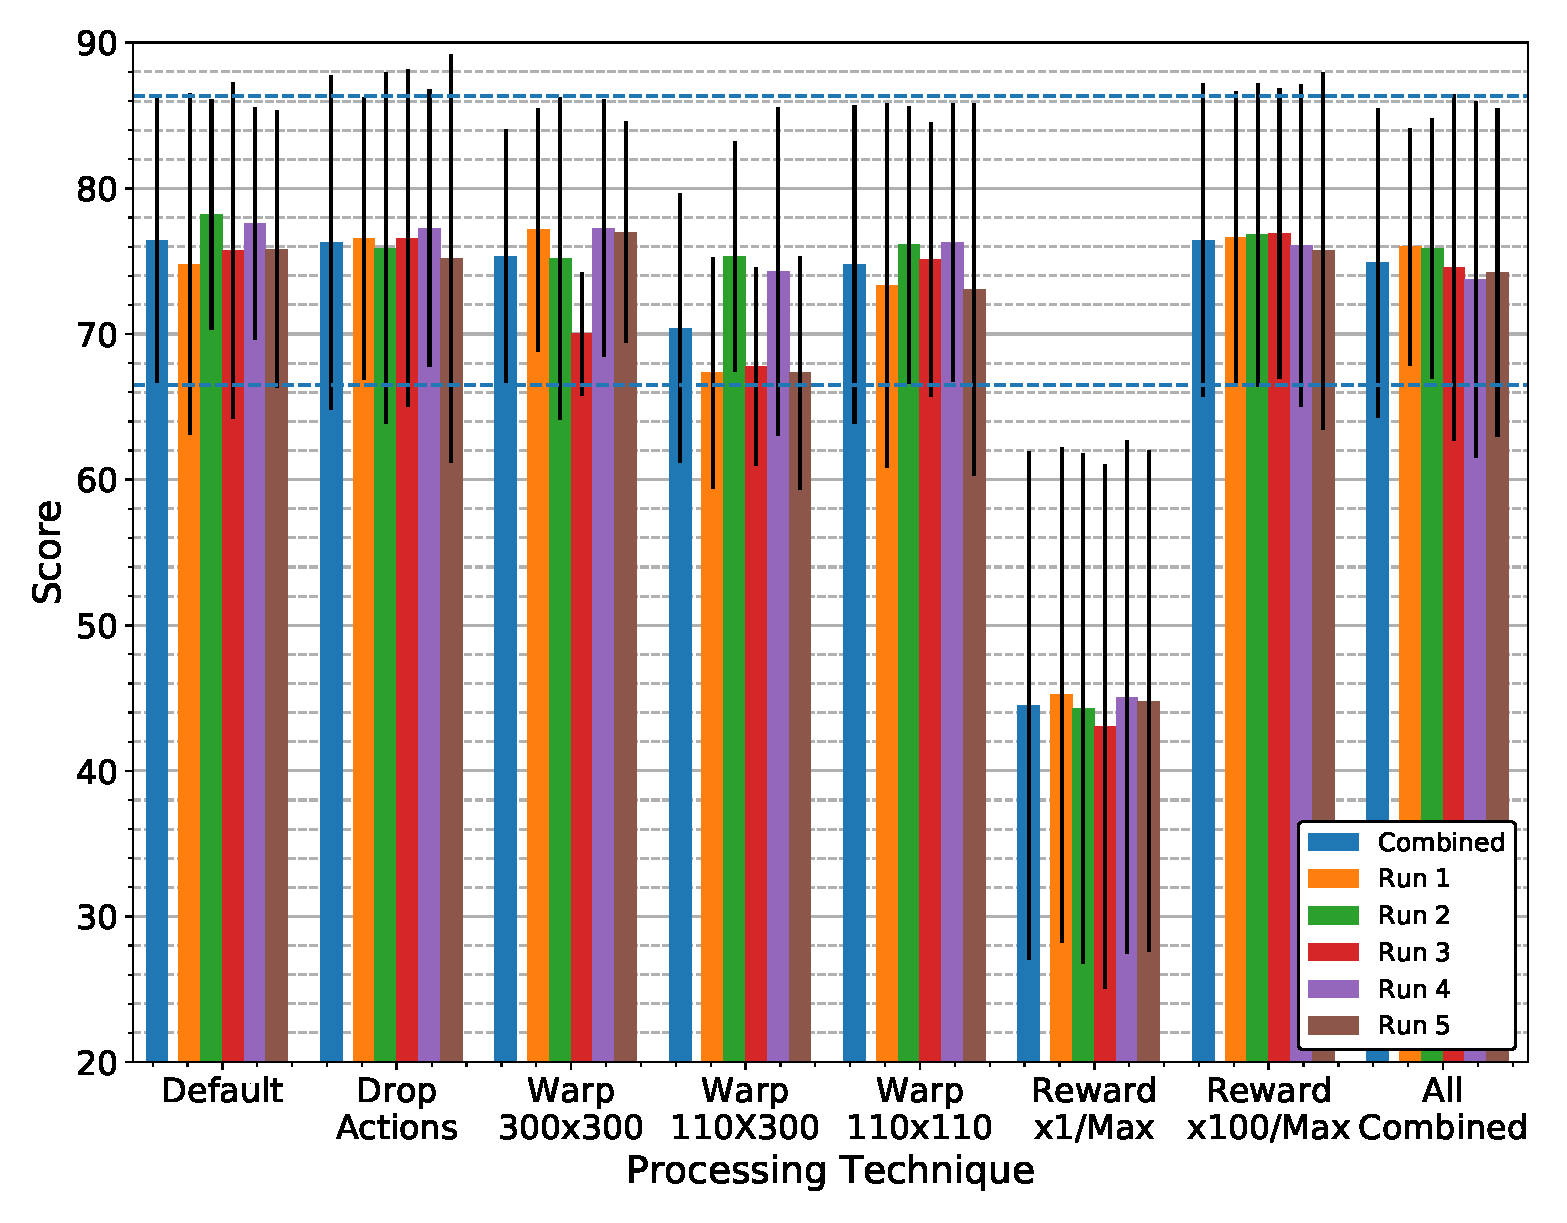
\includegraphics[width=0.45\linewidth]{graphs/Scores.eps} \label{fig:ProcessingA}
  }
  \subfloat[][Win\% w/ $\pm5\%$]{
    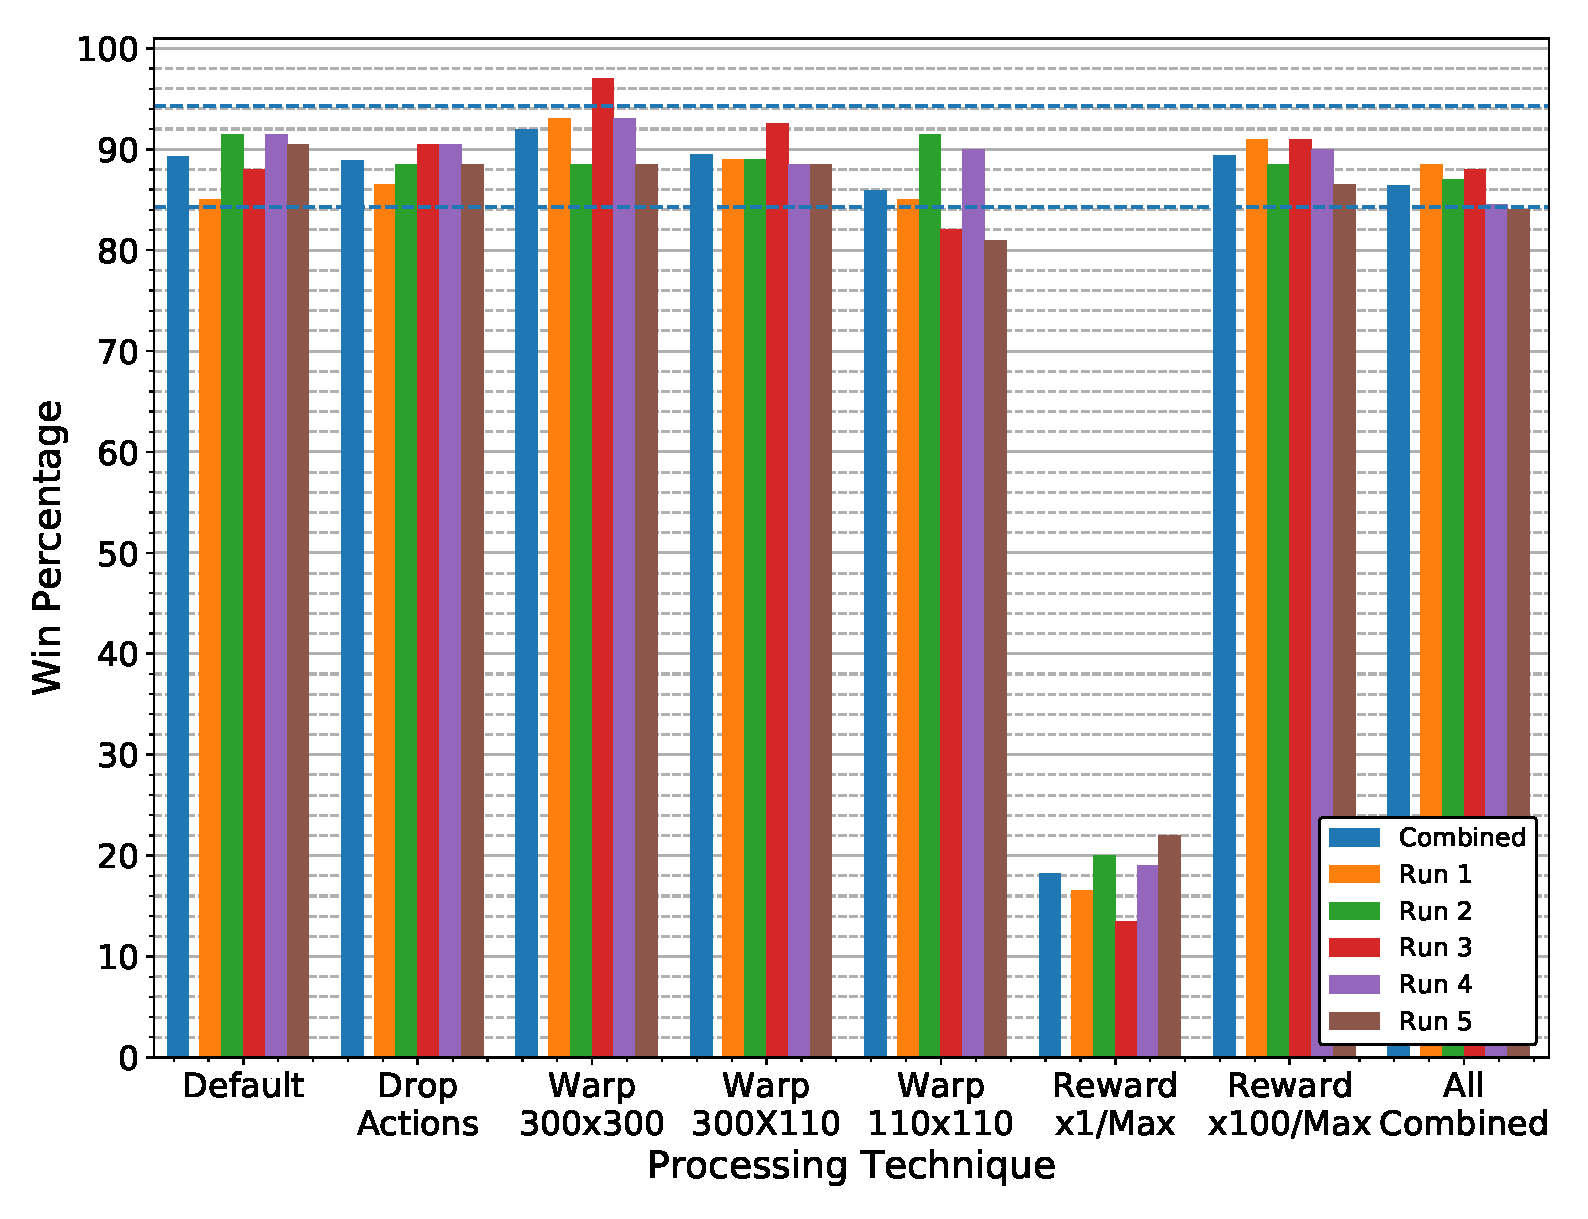
\includegraphics[width=0.45\linewidth]{graphs/Wins.eps} \label{fig:ProcessingB}
  }
  \caption{Performance Comparisons of the Different Methods Tested}
  \label{fig:Processing}
\end{figure*}
The main 3 methods presented were tested to show they aren't negatively effecting performance of the agent when trained with these adaptations. 
Due to the simplicity of the technique, removal of the alpha channel was applied to all of the experiments.
Each of the methods were tested against a agent trained with default settings, and where possible a few hyperparameters for each method were tried.
A final run was also tested which included a combination of all of the methods together.

\subsection{Experimental Method}
\label{ssec:experimentalMethod}
All of the agents were trained and tested on level 1 of the game aliens, to show that the methods don't effect performance of a agent designed to play a single known level - a known successful application of reinforcement learning.
Level 1 of aliens was chosen as it has properties required to test all of the methods and performance can be loosely compared to the results from the initial investigations by Torrado et al. when applying deep reinforcement learning to the GVGAI framework~\cite{GVGAIGym}. 
While any game could serve a decent test for raw state observation image warping, Aliens also has 4 actions due to no vertical movement and a large maximum score with positive rewards of differing magnitudes.
\par
As a efficient and popular modern reinforcement learning algorithm, Advantage Actor-Critic (A2C) was used to test all of the methods.
The implementation for this algorithm came from the Stable Baseline library, a simpler fork of the OpenAI Baseline library~\cite{stable-baselines}.
The model architecture and other hyperparameters were the same as used by Torrado et al. during their introduction of the GVGAI Gym framework~\cite{GVGAIGym}, apart from training time which was increase to ten million frames of gameplay to allow to results on long term performance and convergence to be seen.
As the convergence process of stochastic gradient descent learning is inherently random, five models with each adaptation were trained.

\subsection{Method Hyperparameters Tested}
This section aims to give a brief explanation of the hyperparameters of each adaptation that was tested.
\subsubsection{Dropping Actions}
Dropping unacceptable actions was tested with a model output of size 6 where as aliens only accepts 4 actions.
\subsubsection{Image Warpping}
Three different screen warps were tested. The original screen size is 300x110 so this was used as the basis for screen decisions.
300x300 allows for no loss of data but creates a much larger model, 110x300 creates the same size of model as default but still warps the image, 110x110 will only warp the image in the y direction squishing it from 300 to 110.
\subsubsection{Scaling Rewards}
Two different reward scaling factors were tested, one by a factor of $\frac{1}{Max}$ and another by $\frac{100}{Max}$.
The maximum possible score for Aliens level 1 was determined to be 87 through analysis of the game rules and level layout.
\subsubsection{All Combined}
\label{sssec:allCombined}
Finally a combination of all the processing techniques were used in a final experiment, with 110x110 used for image warping and $\frac{100}{Max}$ for the reward scaling factor.

\subsection{Results and Evaluation}
\subsubsection{Performance Graphs}
The graphs in Figure~\ref{fig:Processing} shows the average score and win\% of each of the trained models over 100 games played, in the 5 grouped bars for each method.
The preceding bar shows the combined performance when joining the results from all 5 models trained with that adaptation together.
\par
Figure~\ref{fig:ProcessingA} shows that that the majority of the methods used score within 1 standard deviation of the combined default average score.
Similar results can be seen when comparing the win\% in Figure~\ref{fig:ProcessingB}, again the majority of the methods lie with in a narrow margin of the combined default win\% with $\pm$ 5\% being marked on the graph.

\subsubsection{Low Performance of Reward Scaling by $\frac{1}{Max}$}
The only method that performed badly was scaling the rewards by $\frac{1}{Max}$, with it clearly being an outlier to all the other methods and the default configuration.
The resulting agent performs similarly to a purely random agent, and looking at training metrics it suggests that the model struggled to learn throughout the training process.
This could be attributed to vanishing gradients during training, this occurs when the weight updates for each minibatch are insignificant and the model doesn't learn due to the small gradients received, which could be due to the small rewards given.
Changing hyperparameters such as learning rate could mitigate this but as a reward scaling of $\frac{100}{Max}$ has proven to be effective this wasn't investigated.
\subsubsection{Conclusion}
These results show that these methods do not negatively impact performance on single game playing.
By using the combination of input and output processing, any game can be processed by the model to allow GVGP, while employing reward scaling cross game training can happen more effectively.
